\section*{Lezione 9}
\addcontentsline{toc}{section}{Lezione 9}

\subsection*{Teoria dell'informazione - Entropia}
\addcontentsline{toc}{subsection}{Teoria dell'informazione - Entropia}

Prendiamo una sorgente $S = {s_1, s_2, ..., s_q}$ caratterizzato dalle probabilità $p_1, p_2, ... , p_q$.
Definiamo una funzione $I(s_i) / I(p_i)$ come la quantità di informazione data da un simbolo.
La quantità di informazione è proporzionale alla "sorpresa" che abbiamo nel leggere il simbolo.

Dominio:
\begin{equation*}
I:S\rightarrow {\rm I\!R}
\end{equation*} 

Inversamente proporzionale alla probabilità:
\begin{equation*}
I(p_i) = \frac{1}{p_i}
\end{equation*}

Abbiamo bisogno inoltre della proprietà additiva: l'informazione di due eventi stocastici indipendenti si sommano:
\begin{equation*}
I(p_i) + I(p_j) = \frac{1}{p_i} + \frac{1}{p_j} = \frac{p_j+p_i}{p_ip_j}
\end{equation*}

Ma quello che accade nella realtà è che la probabilità che avvengano due eventi è

\begin{equation*}
I(p_ip_j) = \frac{1}{p_ip_j}
\end{equation*}

Quindi la funzione $I=\frac{1}{p_i}$ non gode della proprietà additiva, quindi la scartiamo.

Cerchiamo di capire come si comporta la funzione che stiamo cercando:
\begin{enumerate}
	\item $I(p) \geq 0 \; \; \; \; \; (positivita)$
	\item $I(p_1p_2) = I(p_1) + I(p_2) \; \; \; \; \; (additivita)$\\
	se gli eventi sono indipendenti
	\item $I \; \text{è una funzione continua di p}$
\end{enumerate}

Notiamo che $I(p^n) = nI(p)$

\textbf{Base induzione:}\\
$I(p) = I(p)$\\
\textbf{Passo induttivo:}\\
Supponiamo che valga $I(p^{n-1}) = (n-1)I(p)$,\\
$I(p^n) = I(pp^{n-1}) = I(p) + I(p^{n-1}) = I(p) + (n-1)I(p) = nI(p)$

\newpage
Ora definiamo $y=p^n$, da cui ricaviamo che $p=y^{\frac{1}{n}}$.
Poi calcoliamo $I(y)=I(p^n)=nI(p)=nI(y^{\frac{1}{n}})$.
\begin{equation*}
I(y^{\frac{1}{n}}) = \frac{1}{n}I(Y) \; \; \; \; \; \; \forall n \in N
\end{equation*}
Ora estendiamo per tutti i numeri razionali:

\begin{equation*}
I(y^{\frac{m}{n}}) = I((y^{\frac{1}{n}})^m) = mI(y^{\frac{1}{n}}) = \frac{m}{n}I(y)
\end{equation*}

Osserviamo queste proprietà, c'è una funzione che le rispetta tutte: il logaritmo.

\begin{equation*}
I(p) = k\cdot \log p
\end{equation*}
per $k=-1$ ottengo:

\begin{empheq}[box=\tcbhighmath]{equation*}
I(p) = \log \frac{1}{p}
\end{empheq}

La proprietà di additività è rispettata:
\begin{equation*}
I(p_1) + I(p_2) = \log \frac{1}{p_1} + \log \frac{1}{p_2} = \log \frac{1}{p_1p_2} = I(p_1p_2)
\end{equation*}

Quale base utilizziamo per il logaritmo? Essa ci fornisce l'unità di misura con cui calcoliamo la quantità di informazione.
La base più utilizzata in natura è $e$, mentre nel mondo digitale si utilizza molto la base 2.


Quanto si calcola in $ln$ l'unità di misura dell'informazione è \textit{nat}, in base 2 l'unità di misura è il \textit{bit}, in base 10 si misura in \textit{Hartley}. In ogni caso posso cambiare base velocemente moltiplicando per una costante $C$.



Ma il logaritmo è l'unica funzione che va bene per rappresentare la funzione $I$?

\begin{dimostrazione}
Fissiamo $I(p)=\log_2\frac{1}{p}$.\\
Abbiamo già visto questa proprietà:
\begin{equation*}
I(p^n)=nI(p)
\end{equation*}
Supponiamo che esista una funzione $g$ per cui $g(p^n)=ng(p)$ che sia continua, e che restituisca valori $\geq 0$.

Proviamo a calcolare la differenza fra il logaritmo e questa ipotetica funzione:

\begin{equation*}
g(p^n) - C \log_2\frac{1}{p^n} = n[g(p)-C\log_2 \frac{1}{p}]
\end{equation*}
Poniamo $C=\frac{g(p_0)}{\log_2\frac{1}{p_0}}$, con $p_0 \neq 0, 1$, quindi diverso dagli estremi. In questo modo la differenza fra le due diventa zero.
\newpage
Ora possono succedere due cose:
\begin{itemize}
	\item Due funzioni completamente diverse:
	\begin{figure}[H]
		\centering
		\includegraphics[width=0.3\linewidth]{immagini/img23}
	\end{figure}
		
	\item Due funzioni che sembrano diverse ma sono la stessa funzione:
	\begin{figure}[H]
		\centering
		\includegraphics[width=0.3\linewidth]{immagini/img24}
	\end{figure}
\end{itemize}

Sfrutto una proprietà dall'analisi matematica per cui ogni numero reale può essere scritto come:

\begin{equation*}
\forall \; z \; \exists \; n \; \; | \; \; z=p_0^n
\end{equation*}

Quindi per $p=p_0$ posso scrivere:

\begin{equation*}
g(z) - C \; log_2\frac{1}{z} = 0
\end{equation*}
Uguale a 0 in quanto $C=\frac{g(p_0)}{\log_2\frac{1}{p_0}}$ annulla l'equazione sopra
\begin{equation*}
g(z) = C \; log_2\frac{1}{z}
\end{equation*}
Quindi questa funzione si dimostra essere un logaritmo
\end{dimostrazione}  

Quindi abbiamo definito l'unica funzione possibile per definire la quantità di informazione per un evento.


Consideriamo una sorgente $S$ che emette $q$ simboli con $p_1, p_2, ..., p_q$.
Abbiamo quindi detto che:
\begin{equation*}
I(s_i)=I(p_i)=log_r\frac{1}{p_i}
\end{equation*}

Quanto è la quantità di informazione media data una sorgente? Chiamo questo valore come $H(s)$.
Per calcolare questo valore peso ogni quantità di informazione:

\begin{equation*}
H(s) = p_1I(s_1) + p_2I(s_2) + ... + p_qI(s_q)
\end{equation*}

Riscriviamo in forma compatta:

\begin{equation*}
H(s) = \sum_{i=1}^qp_iI(s_i)
\end{equation*}

\begin{equation*}
H(s) = \sum_{i=1}^qp_i\log\frac{1}{p_i}
\end{equation*}
oppure scritto come
\begin{equation*}
H(s) = -\sum_{i=1}^qp_i\log{p_i}
\end{equation*}

Questa formula appena scritta è l'\textbf{entropia} di una sorgente ed è definita come:

\begin{empheq}[box=\tcbhighmath]{equation*}
H_r(s) = \sum_{i=1}^qp_i\log_r\frac{1}{p_i}
\end{empheq}

L'unità di misura dell'entropia è data dalla base del logaritmo,
\begin{equation*}
H_r(s) = H_2(s)\log_r2
\end{equation*}
Ma posso cambiare velocemente base tramite una costante.

Se una sorgente fa uscire messaggi lunghi $N$ con simboli $s_q$, mi aspetterò di avere
\begin{itemize}
	\item $N \cdot p_1$ occorrenze di $s_1$
	\item $N \cdot p_2$ occorrenze di $s_2$
	\item ..
	\item $N \cdot p_q$ occorrenze di $s_q$
\end{itemize}

La probabilità $P$ di avere un messaggio fatto in questo modo sarà:
\begin{equation*}
P = p_1^{Np_1} \cdot p_2^{Np_2} \cdot ... \cdot p_q^{Np_q} = [p_1^{p_1}p_2^{p_2}...p_q^{p_q}]^N
\end{equation*}

\newpage 

Quando esce questo messaggio, la quantità di informazione che otteniamo è $\log\frac{1}{p}$, che è quindi:

\begin{equation*}
\log\frac{1}{p} = \log\frac{1}{[p_1^{p_1}p_2^{p_2}...p_q^{p_q}]^N} = \log[\frac{1}{p_1^{p_1}p_2^{p_2}...p_q^{p_q}}]^N = N\log[\frac{1}{p_1^{p_1}} \cdot \frac{1}{p_2^{p_2}} \cdot ... \cdot \frac{1}{p_q^{p_q}}]
\end{equation*}


\begin{equation*}
= N \sum_{i=1}^q\log[\frac{1}{p_i}]^{p_i} = N \sum_{i=1}^qp_i\log\frac{1}{p_i}
\end{equation*}

Quindi l'entropia possiamo vederla come la quantità di informazione mediamente emessa dalla sorgente:

\begin{equation*}
H(s) = \frac{\log\frac{1}{p}}{N}
\end{equation*}

Vediamo ora come è fatta questa funzione entropia:

\begin{figure}[h]
	\centering
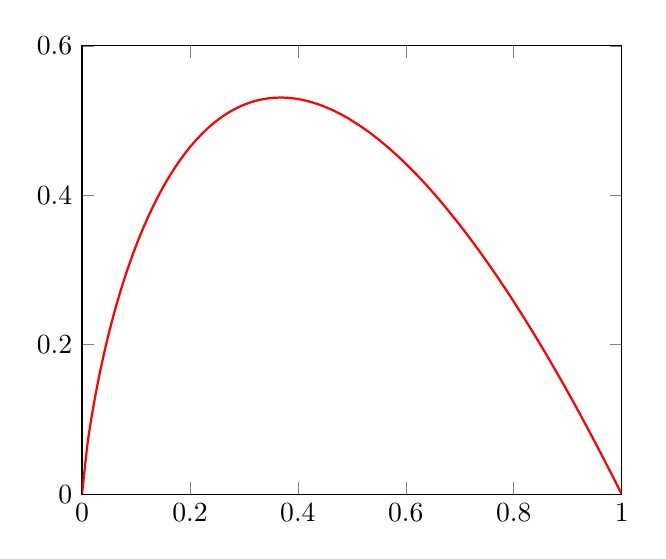
\begin{tikzpicture}
\begin{axis}[
xmin = 0, xmax = 1,
ymin = 0, ymax = 0.6,
]
\addplot[
domain = 0:1,
samples = 100,
smooth,
thick,
red,
] {x*log2(1/x)};
\end{axis}
\end{tikzpicture}
\caption{Grafico funzione $H_2(s)$}
\end{figure}

In $p=0$ abbiamo un punto di discontinuità a cui ci si avvicina con pendenza infinita, quindi definiamo formalmente un'altra funzione per cui se $p=0$ allora la funzione vale 0 (un evento impossibile non ci da informazione).

Il punto massimo vale $\frac{1}{e}$.

L'entropia $H(s)$ è sempre un valore $\geq 0$.\\
Quando vale 0? Essendo una somma di termini $\geq 0$, allora essa si annulla solo se tutti i termini sono uguali a 0, che è il caso in cui la sorgente ha come probabilità $p_1 = 1, p_2 = 0, p_3 = 0, ... p_q = 0$, quindi quando esce sempre lo stesso simbolo.

